\documentclass{beamer}

\mode<presentation>
\usetheme{Warsaw}

\usepackage[OT2]{fontenc}
\usepackage{amsfonts}
\usepackage{amssymb}
\usepackage{amsthm}
\usepackage{amsmath}
\usepackage{newlfont}
\usepackage{graphicx}
\usepackage{multicol}
\usepackage[OT2]{fontenc}
\usepackage{wrapfig}
\usepackage{subcaption}
\usepackage{glossaries}
\usepackage{lipsum}
\usepackage[all,arc]{xy}
\usepackage{epsfig}
\usepackage{pgf}
\usepackage{amscd}
\def \zn{,\kern-0.09em,}
\setlength\intextsep{0pt}
\newcommand\texteng{\fontencoding{OT1}\fontfamily{\rmdefault}\selectfont}
\def\ug{\mathbin{\sphericalangle\,}}
\def\dj{d\kern-0.4em\char"16\kern-0.1em}
\def\Dj{\mbox{\raise0.3ex\hbox{-}\kern-0.4em D}}
\newcommand{\D}{\displaystyle}

\title{Paskalova teorema}
\author{Aleksa Vuchkovic1}
\institute{Matematichka gimnazija}

\date{Mart 2019.}

\setbeamercolor{uppercol}{fg=white,bg=green!75!blue}

\begin{document}
\maketitle

\begin{frame}{Sadrzhaj}
\tableofcontents
\end{frame}

\section{Paskalova teorema}
\begin{frame}{Paskalova teorema}
\onslide<1->
\begin{block}{Teorema}
Neka su $A,B,C,D,E,F$ tachke na krugu. Prave $AB$ i $DE$ seku se u $L$, prave $BC$ i $EF$ u $M$, a $CD$ i $FA$ u $N$. Tada su tachke $L,M,N$ kolinearne.
\end{block}
\vspace{4mm}
\onslide<2->
\begin{block}{}
U projektivnoj geometriji, Paskalova teorema kazhe da ako se izabere shest proizvoljnih tačaka na krugu i da se spoje linijskim segmentima u bilo kom redosledu da formira shestougao, onda se tri para suprotnih strana shestougla sastaju u tri tachke koje lezhe na pravoj liniji.
\end{block}
\end{frame}

\section{Dokaz}
\begin{frame}{Dokaz}
\centering 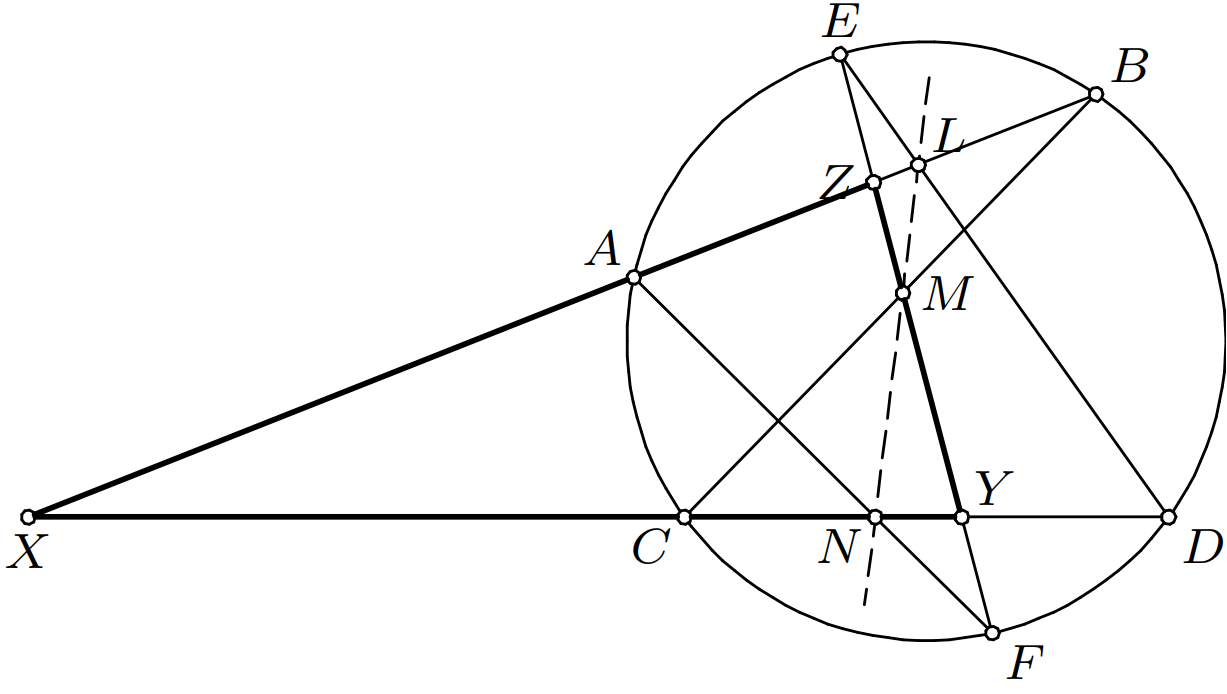
\includegraphics[scale=0.3]{Paskal}
\end{frame}

\section{Posebni sluchajevi}
\begin{frame}{Posebni sluchajevi}
\begin{block}{}
Paskalova teorema oqigledno ne zahteva da $ABCDEF$ bude konveksan shestougao, tako da su svi rasporedi tachaka dozvoljeni. Mozhemo da posmatramo i degenerisane sluchajeve, kada su neke dve prave paralelne ili se neke dve tachke poklapaju. Na primer, ako je $A = B$, za pravu $AB$ uzimamo tangentu na krug u $A$.
\end{block}
\end{frame}

\section{Primena}
\subsection{Zadatak 1.}
\begin{frame}{Zadatak 1.}
\onslide<1->
\begin{block}{}
Neka je $P$ taqka u unutrashnjosti trougla $ABC$. Oznaqimo sa $P_1$ i $P_2$ redom podnozhja
normala iz $P$ na $AC$ i $BC$, i sa $Q_1$ i $Q_2$ redom podnoжja normala iz $C$ na $AP$ i $BP$.
Dokazati da se prave $Q_1P_2$, $Q_2P_1$ i $AB$ seku u jednoj taqki.
\end{block}
\onslide<2->
\centering 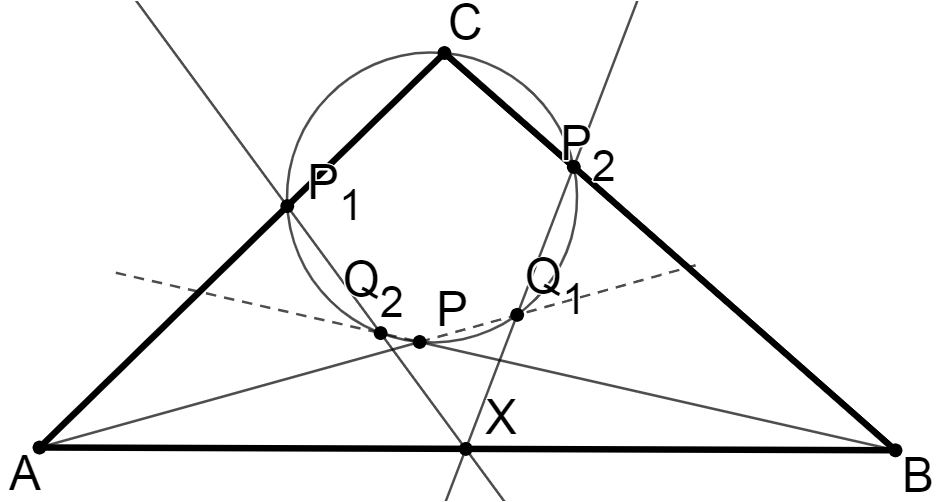
\includegraphics[scale=0.25]{Paskal1}
\end{frame}

\subsection{Zadatak 2.}
\begin{frame}{Zadatak 2.}
\onslide<1->
\begin{block}{}
Trougao $ABC$ je upisan u krug G. Odabrana je taqka $M$ na simetrali ugla $A$, unutar
trougla. Prave $AM$, $BM$ i $CM$ ponovo seku Γ u $A_1$, $B_1$ i $C_1$ redom. Neka prava $A_1C_1$
seqe $AB$ u $P$, a $A_1B_1$ seqe $AC$ u $Q$. Dokazati da je $PQ\parallel BC$.
\end{block}
\onslide<2->
\centering 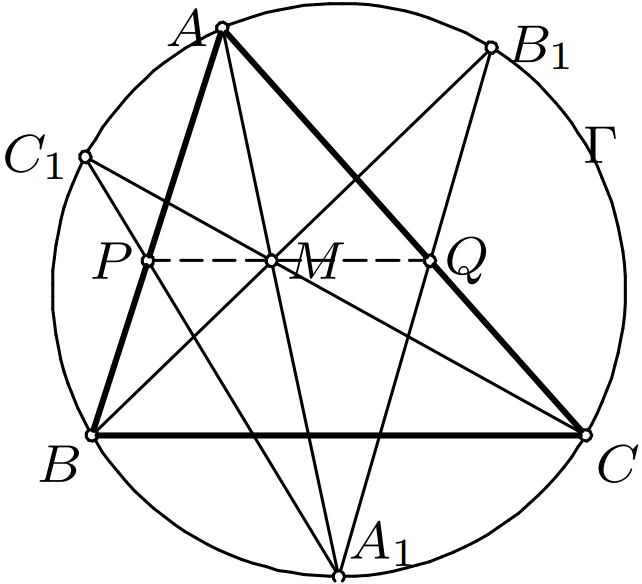
\includegraphics[scale=0.24]{Paskal2}
\end{frame}

\subsection{Zadatak 3.}
\begin{frame}{Zadatak 3.}
\onslide<1->
\begin{block}{}
U trouglu $ABC$, taqke $D$ i $E$ na pravoj $AB$ su takve da je $D-A-B-E$ i $AD = AC$,
$BE = BC$. Oznaqimo sa $M$ i $N$ redom sredixta lukova $AC$ i $BC$ opisanog kruga
$\Delta ABC$ koji ne sadrzhe trec1e teme. Prave $DM$ i $CA$ se seku u $P$, a prave $EN$ i $CB$
se seku u $Q$. Dokazati da centar upisanog kruga $I$ trougla $ABC$ lezhi na pravoj $PQ$.
\end{block}
\onslide<2->
\centering 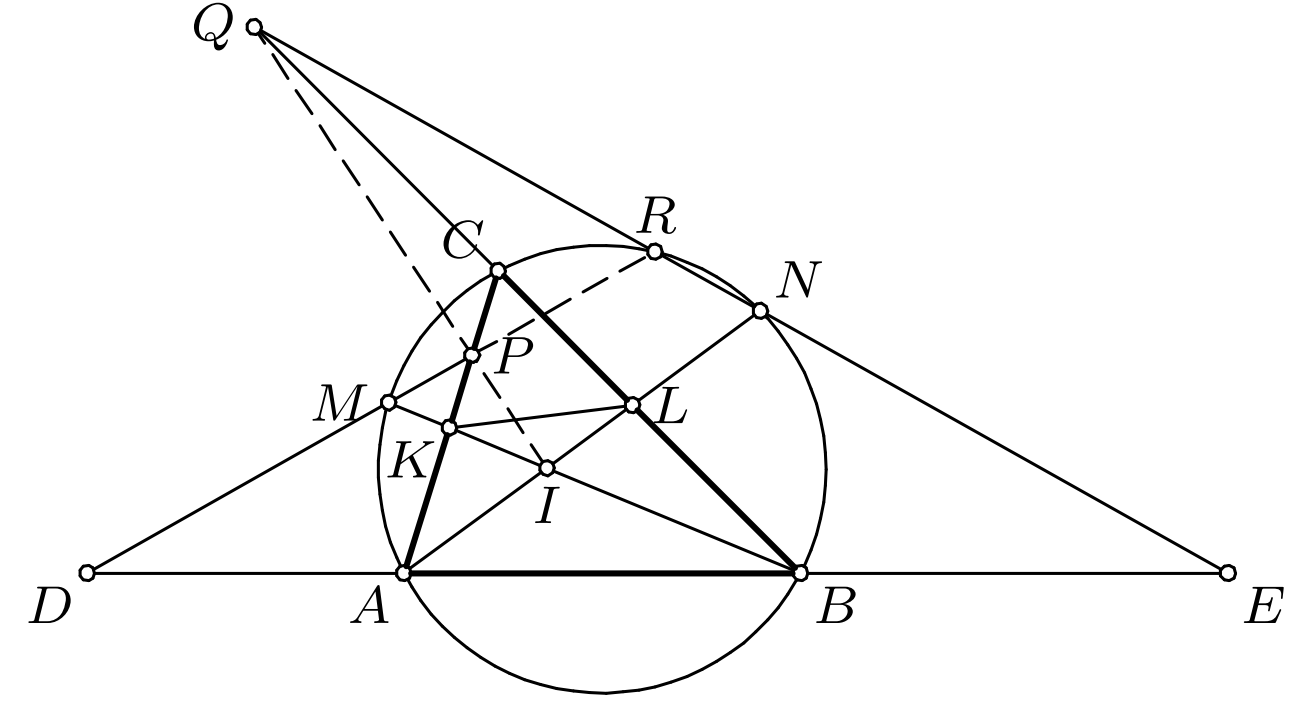
\includegraphics[scale=0.2]{Paskal3}
\end{frame}

\section{}
\begin{frame}
 \centering\LARGE   Hvala na pazhnji!
\end{frame}

\end{document}